\section{Профиль и конфигурация}
\subsection{Цель работы и исследовательские вопросы}
Цель работы --- разработать и проверить единый Experiment Harness для воспроизводимого запуска, регистрации, сравнения и продолжения экспериментов с нейронными сетями. Объект исследования --- вычислительный эксперимент, а компактная свёрточная сеть служит контролируемой моделью. Содержание работы и критерии проверки соответствуют редакции 2.1 задания от 9 октября 2026 г.~\cite{lab0}.

Проверяются три разных утверждения: одинаковые условия дают одинаковый поток данных; повторное обучение воспроизводит траекторию и итоговую метрику; восстановление полного состояния воспроизводит непрерывное обучение. Дополнительно оцениваются разброс качества между случайными инициализациями и вычислительная стоимость модели. Высокая точность сама по себе не является целью инфраструктурного эксперимента.

\subsection{Данные, индивидуальный профиль и модель}
Использован CIFAR-10: цветные изображения $32\times32$ десяти классов~\cite{cifar}. Роли данных фиксируются до обучения; разбиение стратифицировано с seed 1729. Из официальных 50\,000 обучающих изображений выделены 43\,000 для train, 5\,000 для val и 2\,000 для cal. Официальные 10\,000 тестовых изображений образуют test. В Lab~0 используется четверть train, то есть 10\,750 изображений (\run{R01}).

Средние и стандартные отклонения каналов вычислены только по полному train: $(0.491359,\,0.482010,\,0.446343)$ и $(0.246676,\,0.243134,\,0.261255)$. Каждый канал преобразуется по правилу $x'_c=(x_c-\mu_c)/\sigma_c$. Эти величины не пересчитываются на val, cal или test. В данной работе cal и test не использованы; все приведённые показатели качества относятся к val. Отдельный файл протокола данных курса отсутствует, поэтому совпадение индексов с независимым файлом преподавателя не установлено. Численности ролей и правило их построения соответствуют заданию.

Профиль \texttt{P3adf02} вычислен из SHA256 идентификатора студента по правилам §11 задания. В репозитории сохраняется хеш идентификатора, исходный номер не публикуется. Полученные значения и фактические условия приведены в табл.~\ref{tab:config}; они взяты из разрешённой конфигурации \run{R01}, а не из демонстрационного YAML.

\begin{table}[H]
\centering\small
\caption{Индивидуальная конфигурация и фиксированные условия (\run{R01}).}\label{tab:config}
\begin{tabular}{@{}p{6.4cm}p{8.4cm}@{}}
\toprule Параметр & Значение \\\midrule
Профиль / базовый seed & \texttt{P3adf02} / 987693601 \\
Доля train / число объектов & 0.25 / 10\,750 \\
Модель / число параметров & SmallCNN / 252\,778 \\
Ширина / глубина & 96 каналов / 4 свёрточных слоя \\
Размер mini-batch & 64 \\
Оптимизатор & AdamW, $\eta_0=0.001$, weight decay $10^{-4}$ \\
Расписание скорости обучения & Cosine, одна эпоха прогрева \\
Число эпох / накопление градиентов & $K=12$ / 1 mini-batch \\
Параллельная загрузка / потоки CPU & \texttt{num\_workers}=0 / 2 \\
Batch sizes профилирования & $1,16,64,256$ \\
Аугментации / BatchNorm / dropout & Отсутствуют \\
\bottomrule
\end{tabular}
\end{table}

Сеть содержит четыре Conv2d $3\times3$ с шагом 1, padding 1 и смещением; после каждой свёртки применяется ReLU. После первых трёх свёрток используется MaxPool2d $2\times2$. Все скрытые слои имеют 96 каналов. Затем следуют глобальное усреднение по пространству и Linear $96\to10$. Изменение seed не меняет архитектуру, данные, нормализацию и бюджет.

\subsection{Вычислительное окружение и бюджет}
Архивные запуски выполнены с Python 3.11.17, PyTorch 2.7.1+cu126, CUDA 12.6 и cuDNN 90701 на Windows; GPU --- NVIDIA GeForce RTX 3060 Laptop с 6~GB памяти. В режиме A используется CPU с детерминированными алгоритмами, без AMP и с workers=0; B отличается использованием CUDA; C использует CUDA и AMP. Опыт с workers=2 рассматривается отдельно как ослабление условий режима A. Одинаковый seed не гарантирует совпадения CPU и GPU или разных версий библиотек~\cite{torch}.

В бюджетном запуске \run{D01} измерено $T_{\text{эп}}=24.0901$~с, что меньше предела 60~с. При $K=12$ оценка обязательной CPU-программы составляет
\begin{equation}
T_{\text{полн}}\approx13KT_{\text{эп}}
=13\cdot12\cdot24.0901=3758.06\text{ с}\approx62.63\text{ мин}.
\label{eq:budget}
\end{equation}
Коэффициент 13 учитывает логические траектории, перечисленные в задании; прерванная и возобновлённая части не считаются двумя независимыми полными обучениями. Основная последовательная серия заняла 65.05~мин по журналу серии; ранее выполненный E0, позднейшие дополнительные seeds и профилирование не входят в этот интервал. Режимы B/C исследованы дополнительно.

Исходная попытка E0 с $K=10$ не прошла порог уменьшения loss вдвое (см. §\ref{sec:e0}). До основной серии бюджет увеличен до 12 эпох с обучением заново. Значения индивидуального профиля не изменены; увеличение $K$ не выдаётся за успешность исходного десятиэпохового опыта.

\section{Устройство harness}
\subsection{Теоретическая модель эксперимента}
Эксперимент задаётся кодом $C$, разрешённой конфигурацией $\Theta$, данными и разбиением $D$, состоянием случайности $S$ и окружением $V$:
\begin{equation}
R=(C,\Theta,D,S,V),\qquad
\mathcal A=\{M,L,P,K,T\}.
\label{eq:experiment}
\end{equation}
Здесь $\mathcal A$ --- артефакты; $M$ --- метрики, $L$ --- журналы, $P$ --- графики, $K$ --- контрольные точки, $T$ --- временные и ресурсные характеристики. Два результата сопоставимы лишь после проверки условий, в которых они получены.

Для классификации минимизируется средняя перекрёстная энтропия:
\begin{equation}
\mathcal L_B(\theta)=-\frac{1}{B}\sum_{i=1}^{B}
\log\frac{\exp z_{i,y_i}}{\sum_{c=1}^{10}\exp z_{i,c}},\qquad
\operatorname{acc}=\frac{1}{n}\sum_{i=1}^{n}
\mathbf1\!\left[\arg\max_c z_{i,c}=y_i\right].
\label{eq:loss}
\end{equation}
$z_{i,c}$ --- логит класса $c$, $y_i$ --- истинная метка, $B$ --- размер mini-batch, $n$ --- число объектов при оценивании. Эпохальная loss усредняется с весом по числу объектов, поэтому последний неполный mini-batch не получает завышенного веса. Регуляризация AdamW задаётся параметром weight decay отдельно от записываемой cross-entropy.

Для $N$ запусков с различными seed вычисляются
\begin{equation}
\overline m=\frac{1}{N}\sum_{i=1}^{N}m_i,\qquad
s_m=\sqrt{\frac{1}{N-1}\sum_{i=1}^{N}(m_i-\overline m)^2},
\label{eq:statistics}
\end{equation}
\begin{equation}
\operatorname{CI}_{95\%}(\overline m)=
\overline m\pm t_{0.975,N-1}\frac{s_m}{\sqrt N}.
\label{eq:ci}
\end{equation}
$m_i$ --- итоговая val accuracy отдельного запуска, $s_m$ --- выборочное стандартное отклонение, $t_{0.975,N-1}$ --- квантиль распределения Стьюдента. Интервал описывает неопределённость среднего по seed при фиксированном split; он не учитывает смену обучающей выборки и не является диапазоном для любого будущего запуска.

\subsection{Семь компонентов и регистрация условий}
Общий runner связывает семь компонентов (рис.~\ref{fig:harness}). Конфигурация отделена от модели и цикла обучения. До запуска формируется resolved config, после чего фиксируются идентичность данных и условия вычислений. Основной цикл независимо вызывает обучение и validation; отдельное оценивание загружает сохранённый checkpoint.

\begin{figure}[H]
\centering
\begin{tikzpicture}[node distance=6mm,box/.style={draw,rounded corners=1pt,align=center,text width=4.0cm,minimum height=11mm,font=\small},>=stealth]
\node[box] (a) {1. Разрешённая\\конфигурация};
\node[box,right=of a] (b) {2. Данные, split\\и нормализация};
\node[box,right=of b] (c) {3. Построение\\модели};
\node[box,below=of c] (d) {4. Оптимизатор\\и scheduler};
\node[box,left=of d] (e) {5. ExperimentRunner\\и обучение};
\node[box,left=of e] (f) {6. Validation\\и evaluation};
\node[box,below=of f] (g) {7. Артефакты\\и итоговые метрики};
\draw[->] (a)--(b);\draw[->](b)--(c);\draw[->](c)--(d);\draw[->](d)--(e);\draw[->](e)--(f);\draw[->](f)--(g);
\end{tikzpicture}
\caption{Схема единого Experiment Harness. Для всех условий используется общий цикл обучения.}\label{fig:harness}
\end{figure}

Идентичность условий и идентичность отдельного запуска разделены:
\begin{equation}
\begin{aligned}
\mathrm{EXP\_ID}&=H(C,\Theta,D,S),\\
\mathrm{RUN\_ID}&=\mathrm{EXP\_ID}\,\Vert\,\mathrm{UUID}.
\end{aligned}\label{eq:ids}
\end{equation}
$H$ --- SHA256 канонического описания; в имени используется префикс из 20 шестнадцатеричных символов. $\Vert$ обозначает конкатенацию. В $C$ учитываются версия и состояние исходного кода; в $D$ --- содержимое данных и split. Окружение $V$ сохраняется отдельно и не включается в EXP\_ID. Поэтому одинаковый EXP\_ID означает одинаковые заявленные условия, но не доказывает совпадения вычислений после смены устройства или библиотеки.

Manifest хранит оба идентификатора, профиль и его хеш, seed, разрешённую конфигурацию, происхождение кода и данных, версии библиотек, устройство и число параметров. Журналы сохраняют train/val loss и accuracy, learning rate, epoch, global step, время эпохи и loss каждого mini-batch. Повторный запуск получает новую директорию и не заменяет предыдущий.

Вместо внешнего сервиса выбран локальный машиночитаемый журнал: это позволяет восстановить таблицы без доступности стороннего аккаунта. Малые текстовые артефакты и split версионируются; большие данные, графические кэши и веса хранятся отдельно. Без checkpoint остаётся описание опыта и возможность переобучения, но теряется готовое состояние модели и оптимизатора для немедленного точного продолжения.

Проверка инфраструктуры охватывает разрешение конфигурации, неизменность split при одинаковом seed, сохранение предсказаний при загрузке checkpoint, детерминированность метрик, чувствительность EXP\_ID к существенным условиям и уникальность RUN\_ID. Отдельно проверены отсутствие перезаписи результатов, учёт изменений кода, воспроизводимость профиля, смена профиля без редактирования training code и конфигурационный выбор CPU/CUDA. Эти проверки подтверждают инварианты реализации; реальные эксперименты E0--E4 ниже проверяют её поведение на CIFAR-10.

\subsection{Методика повторения и восстановления}
Фиксируются генераторы Python, NumPy, Torch и CUDA, отдельный generator загрузчика и seed каждого worker. Используются детерминированные алгоритмы, отключён подбор алгоритмов cuDNN; параметры TF32 и вычислительное окружение регистрируются. Эти меры ограничивают источники вариативности в данном окружении, но не устраняют неассоциативность операций с плавающей точкой и различия реализаций между платформами~\cite{torch}.

Полный checkpoint содержит веса, состояния optimizer и scheduler, номер эпохи и число фактических обновлений, генераторы случайных чисел, generator загрузчика и GradScaler при AMP. Продолжение реализовано на границе законченной эпохи. Сначала восстанавливается логическая позиция, затем начинается следующая эпоха; родительский и дочерний запуски имеют разные RUN\_ID.

Для сравнения траекторий и параметров применяются величины задания:
\begin{equation}
\varepsilon_{rel}(x,y)=\frac{|x-y|}{\max(1,|x|)},\qquad
\Delta_\theta=\frac{\|\theta_A-\theta_B\|_2}{\|\theta_A\|_2+10^{-12}}.
\label{eq:distances}
\end{equation}
$x,y$ --- соответствующие значения loss; $\theta_A,\theta_B$ --- векторы всех параметров после одинакового бюджета. При AMP шаг, пропущенный из-за overflow, не увеличивает счётчик обновлений оптимизатора. Поэтому число обработанных mini-batch и число обновлений могут различаться.

\section{Результаты E0--E4}
Во всех таблицах используются точности на validation, а обозначения \run{R01}--\run{R27}, \run{D01}--\run{D08} раскрываются в приложении, табл.~\ref{tab:runs}. Они являются ссылками на конкретные RUN\_ID, а не усреднёнными или синтетическими примерами. Графики построены заново из сохранённых журналов без повторного обучения.

\subsection{E0. Проверка обучаемости baseline}\label{sec:e0}
Цель E0 --- убедиться, что baseline действительно обучается, а сохранённый результат доступен отдельному оцениванию. Для окончательной конфигурации выполнены 12 эпох (\run{R01}). Значения первой и последней эпох приведены в табл.~\ref{tab:e0}; динамика трёх режимов показана на рис.~\ref{fig:learning}.

\begin{table}[H]\centering\small
\caption{Первый и последний этапы обучения E0 (\run{R01}).}\label{tab:e0}
\begin{tabular}{lrr}
\toprule
Показатель & Эпоха 1 & Эпоха 12 \\
\midrule
Train loss & 1.964259 & 0.895176 \\
Val loss & 1.728248 & 1.051922 \\
Train accuracy & 0.258512 & 0.680000 \\
Val accuracy & 0.346400 & 0.623200 \\
\bottomrule
\end{tabular}

\end{table}

Отношение итоговой train loss к loss первой эпохи составляет $0.895176/1.964259=0.455732<0.5$. Val accuracy равна $0.6232>0.30$ и заметно выше случайного угадывания $0.10$. Все 12 эпох записаны; отдельный evaluate по последнему checkpoint воспроизвёл accuracy $0.6232$ с нулевым расхождением. Таким образом, окончательный E0 удовлетворяет порогам задания.

Начальный десятиэпоховый опыт \run{D02} дал $1.964259\to0.982782$, отношение $0.500332>0.5$: исходный порог не выполнен. Значение близко к границе, однако округление не превращает его в успешный результат. Двенадцатиэпоховый E0 является новым обучением с другим расписанием, а не переименованием этой попытки.

\begin{figure}[H]\centering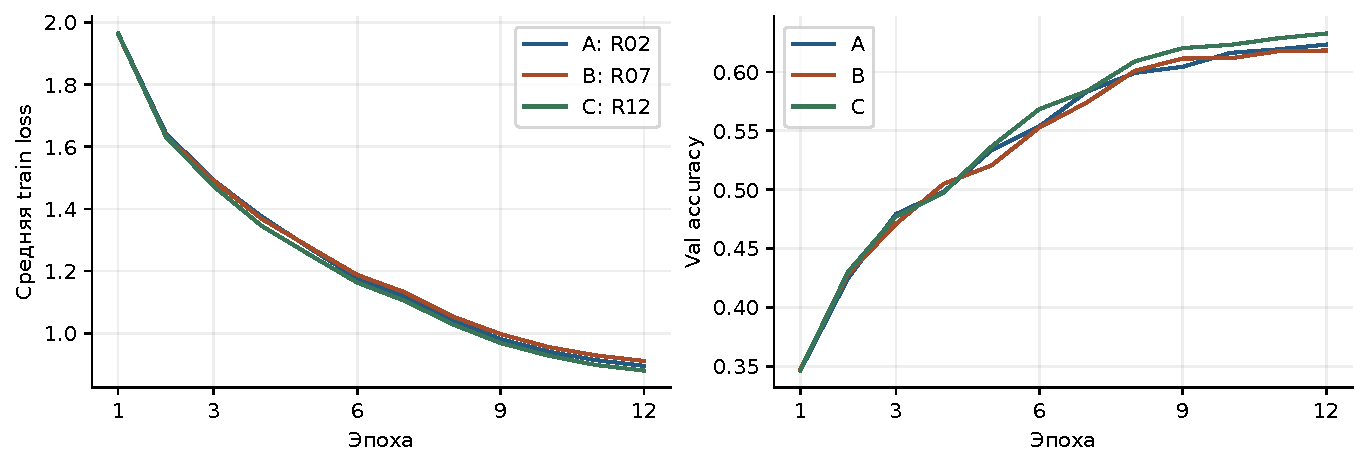
\includegraphics[width=\linewidth]{figures/learning_curves.pdf}
\caption{Train loss и val accuracy в режимах A/B/C (\run{R02}, \run{R07}, \run{R12}). Между устройствами точное совпадение не ожидается.}\label{fig:learning}
\end{figure}

\subsection{E1. Повторный запуск при одинаковом seed}
Для каждого режима выполнены два независимых запуска с одинаковым seed 987693601. Совпали EXP\_ID, разрешённая конфигурация, split и checksum первого batch; RUN\_ID различны. Сравнение всех 2016 записей loss, а не только последних метрик, приведено в табл.~\ref{tab:e1} и на рис.~\ref{fig:repeat}.

\begin{table}[H]\centering\small
\caption{Повторяемость двух независимых запусков E1.}\label{tab:e1}
\begin{tabular}{llrrr}
\toprule
Режим & Запуски & Mini-batch & Макс. $\varepsilon_{rel}$ & $|\Delta acc|$ \\
\midrule
A & R02, R03 & 2016 & 0 & 0 \\
B & R07, R08 & 2016 & 0 & 0 \\
C & R12, R13 & 2016 & 0 & 0 \\
\bottomrule
\end{tabular}

\end{table}

В режиме A требуются нулевые расхождения loss и итоговой метрики: оба условия выполнены. В режиме B допустимы $\varepsilon_{rel}\le10^{-5}$ и разность accuracy не более $0.001$; измеренные расхождения также равны нулю. В режиме C численные пороги не нормируются: точное совпадение здесь является наблюдением, требующим объяснения, а не общей гарантией AMP.

\begin{figure}[H]\centering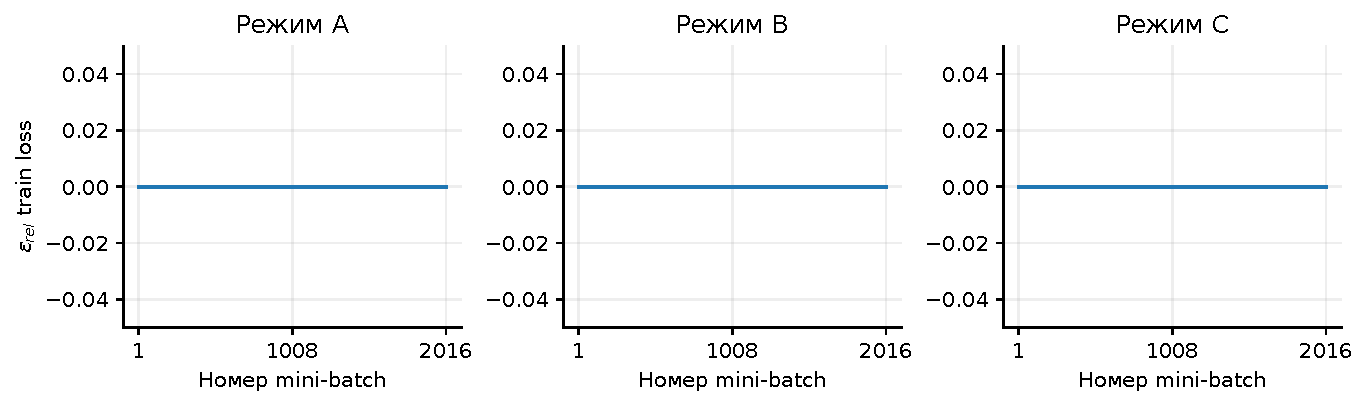
\includegraphics[width=\linewidth]{figures/repeatability.pdf}
\caption{Поэлементное сравнение train loss: \run{R02}/\run{R03}, \run{R07}/\run{R08}, \run{R12}/\run{R13}. Нулевая линия означает совпадение всех сохранённых значений.}\label{fig:repeat}
\end{figure}

В C сохранены одинаковые seed, порядок данных, устройство и выбор алгоритмов. Смешанная точность сама по себе не добавляет случайность; последовательность масштабирования градиента также воспроизвелась. Поэтому в данном pipeline отсутствие расхождения совместимо с ограниченными гарантиями режима C. Оно не доказывает повторяемость любых AMP-экспериментов.

\subsection{E2. Вариативность между seed}
Для E2 заранее использовано правило $s_k=987693601+k$, $k=0,\ldots,4$. Архитектура, split, нормализация, optimizer и число эпох фиксированы; меняются инициализация и определяемый seed порядок обучения. Все пять результатов приведены в табл.~\ref{tab:seeds}; ни один seed не исключён.

\begin{table}[H]\centering\small
\caption{Полная основная серия E2: пять seed в режиме A.}\label{tab:seeds}
\begin{tabular}{lrrrr}
\toprule
Запуск & Seed & Train loss & Val loss & Val accuracy \\
\midrule
R17 & 987693601 & 0.895176 & 1.051922 & 0.6232 \\
R18 & 987693602 & 0.793871 & 1.009430 & 0.6448 \\
R19 & 987693603 & 0.865905 & 1.036181 & 0.6320 \\
R20 & 987693604 & 0.803098 & 1.003634 & 0.6394 \\
R21 & 987693605 & 0.859519 & 1.050276 & 0.6278 \\
\bottomrule
\end{tabular}

\end{table}

По формулам~\eqref{eq:statistics}--\eqref{eq:ci} получены
\begin{equation}
\overline m=0.633440,\quad s_m=0.008708,\quad
\operatorname{CI}_{95\%}=[0.622628;\,0.644252],\quad N=5.
\label{eq:observed}
\end{equation}
Использован $t_{0.975,4}=2.776445$. В процентах результат равен $(63.344\pm0.871)\%$; стандартное отклонение меньше заданного ориентира 1.5 процентного пункта. Эвристический масштаб различимого эффекта $2s_m=0.017416$, то есть 1.742 п.п. Разница между лучшим и худшим seed составляет 2.16 п.п., поэтому выбор только лучшего запуска дал бы завышенное представление о типичном качестве.

\begin{figure}[H]\centering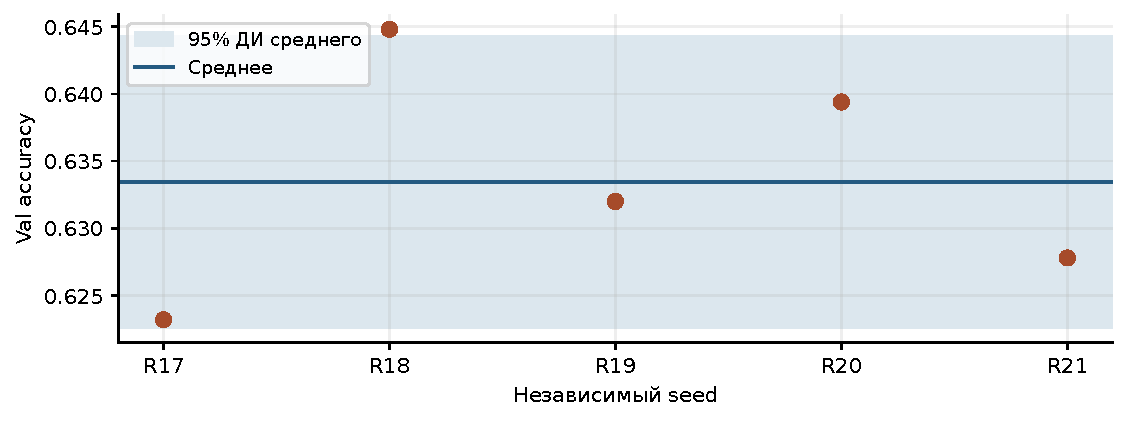
\includegraphics[width=.88\linewidth]{figures/seed_variance.pdf}
\caption{Пять наблюдений E2 и 95\%-й доверительный интервал среднего (\run{R17}--\run{R21}). Полоса не является интервалом предсказания отдельного запуска.}\label{fig:seeds}
\end{figure}

Разброс возникает при одинаковом split: он связан с обучением, а не со случайным разделением данных. Результат не обосновывает преимущество новой архитектуры на один процентный пункт по одному seed; для такой гипотезы необходима отдельная согласованная серия.

\subsection{E3. Эквивалентность checkpoint/resume}
Сравнивались непрерывное обучение 12 эпох и обучение 6 эпох с завершением процесса, загрузкой полного checkpoint в новом процессе и продолжением до 12 эпох. Во всех режимах сравниваются одинаковые последовательности mini-batch и итоговое состояние; результаты приведены в табл.~\ref{tab:resume} и на рис.~\ref{fig:resume}.

\begin{table}[H]\centering\small
\caption{E3: непрерывный, прерванный и возобновлённый запуски.}\label{tab:resume}
\begin{tabular}{llrrrr}
\toprule
Режим & Непр./прер./resume & Обновления & Пропуски & $\Delta_\theta$ & Val acc. \\
\midrule
A & R04/R05/R06 & 2016 & 0 & 0 & 0.6232 \\
B & R09/R10/R11 & 2016 & 0 & 0 & 0.6182 \\
C & R14/R15/R16 & 2015 & 1 & 0 & 0.6326 \\
\bottomrule
\end{tabular}

\end{table}

В A получено $\Delta_\theta=0\le10^{-7}$, в B --- $0\le10^{-5}$. Итоговая accuracy совпала; все сохранённые step loss также совпали. Число фактических обновлений одинаково между непрерывной и восстановленной траекториями: 2016 в A/B и 2015 в C. В C один из 2016 mini-batch привёл к overflow и пропуску обновления в обеих траекториях. Это зарегистрированное поведение GradScaler, а не потерянный шаг после восстановления.

\begin{figure}[H]\centering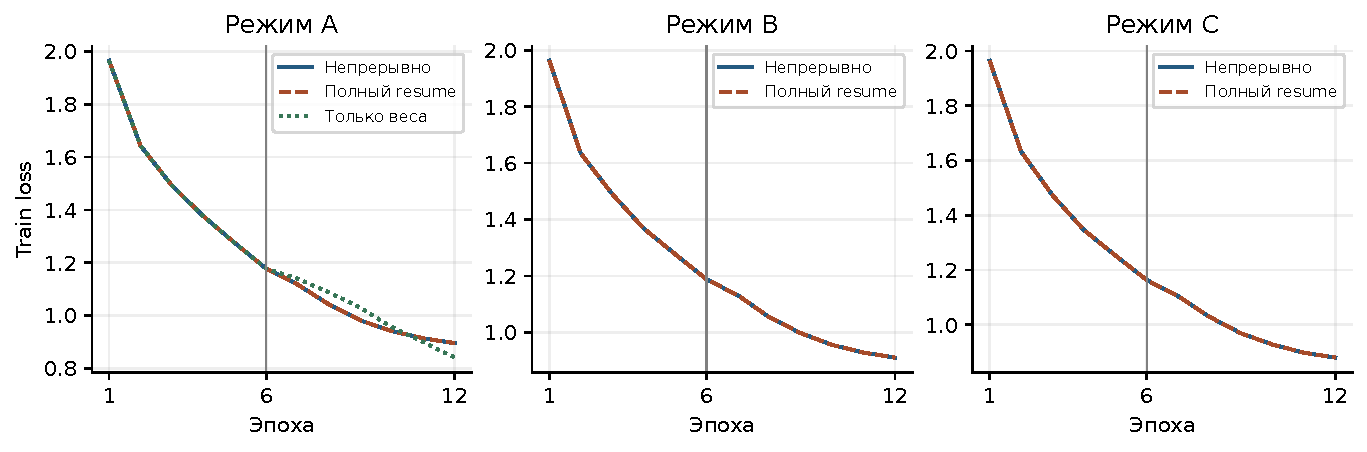
\includegraphics[width=\linewidth]{figures/resume_and_ablation.pdf}
\caption{Непрерывная и восстановленная траектории E3: \run{R04}--\run{R06}, \run{R09}--\run{R11}, \run{R14}--\run{R16}. В A дополнительно показан resume только весов (\run{R24}); пунктир полного resume накладывается на непрерывную кривую.}\label{fig:resume}
\end{figure}

Сохранение полного состояния, включая данные optimizer и generator загрузчика, достаточно для точного продолжения на границе эпохи в исследованном окружении. Загрузка только весов дала $\Delta_\theta=0.371028$ (\run{R24}); причины этой разницы отдельно разобраны в вопросе~\ref{cf:3}. Таким образом, обычный перенос обученных весов и точное продолжение эксперимента --- разные операции.

\subsection{E4. Latency, throughput и потребление памяти}
Профилировалась та же сеть с весами \run{R02}. Для каждого $B\in\{1,16,64,256\}$ выполнены 50 прогревочных и 100 измеряемых forward pass; перед и после каждого GPU-интервала выполнялась синхронизация. Входы имеют форму $B\times3\times32\times32$ и являются явно заданными случайными тензорами: это измерение производительности, а не качества классификации. CPU-серия имеет RUN\_ID \run{D06}, CUDA-серия --- \run{D07}.

При временах $t_j$ пропускная способность и коэффициент вариации определяются как
\begin{equation}
Q(B)=\frac{B}{\overline t(B)},\qquad
\mathrm{CV}(B)=\frac{s_t(B)}{\overline t(B)}.
\label{eq:performance}
\end{equation}
Здесь $\overline t$ и $s_t$ --- среднее и выборочное стандартное отклонение времени batch, $Q$ измеряется в объектах/с. Throughput каждого $B$ рассчитан по собственным измерениям. Показатели forward pass не включают backward и optimizer step.

\begin{table}[H]\centering\fontsize{9.2}{12}\selectfont\setlength{\tabcolsep}{4pt}
\caption{Основные измерения E4, 100 повторов после прогрева (\run{D06}, \run{D07}).}\label{tab:perf}
\begin{tabular}{lrrrrrrr}
\toprule
Устр. & $B$ & Сред., мс & Мед., мс & $p_{95}$, мс & Объект/с & CV, \% & MiB \\
\midrule
CPU & 1 & 1.1572 & 1.1524 & 1.1914 & 864.12 & 1.63 & --- \\
CPU & 16 & 13.6443 & 13.5893 & 14.2845 & 1172.65 & 2.19 & --- \\
CPU & 64 & 53.6907 & 53.5572 & 54.7072 & 1192.01 & 1.01 & --- \\
CPU & 256 & 215.7320 & 214.8388 & 219.6980 & 1186.66 & 1.58 & --- \\
CUDA & 1 & 0.6578 & 0.6619 & 0.6797 & 1520.19 & 2.36 & 34.04 \\
CUDA & 16 & 1.2995 & 1.2944 & 1.3372 & 12312.81 & 1.91 & 45.15 \\
CUDA & 64 & 1.5343 & 1.5352 & 1.5776 & 41711.69 & 3.81 & 81.72 \\
CUDA & 256 & 5.1167 & 5.1001 & 5.1928 & 50032.69 & 1.73 & 227.97 \\
\bottomrule
\end{tabular}

\end{table}

\begin{figure}[H]\centering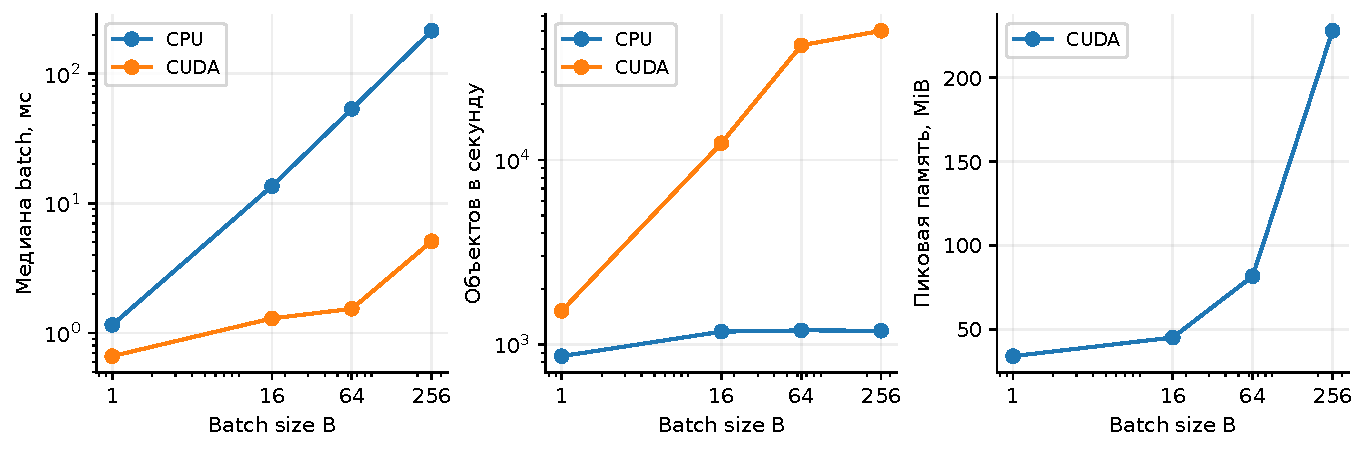
\includegraphics[width=\linewidth]{figures/performance.pdf}
\caption{Медианная latency batch, throughput и пиковая выделенная GPU-память в основной серии E4 (\run{D06}, \run{D07}). Память относится к forward pass.}\label{fig:perf}
\end{figure}

Во всех основных условиях CV меньше 10\%; приведены среднее, медиана и $p_{95}$. Для CPU наименьшая медианная latency достигается при $B=1$, а максимальный наблюдаемый throughput --- при $B=64$. На GPU throughput продолжает расти до $B=256$, тогда как память увеличивается с 34.04 до 227.97~MiB. Больший batch повышает загрузку вычислительных блоков и распределяет накладные расходы, но требует больше памяти и увеличивает время ожидания целого batch. Поэтому оптимум latency и максимум throughput различаются.

Время полной эпохи с validation измерено по журналам обучения (табл.~\ref{tab:epoch}). Оно включает обучение и оценивание, поэтому отличается от времени forward pass.

\begin{table}[H]\centering\small
\caption{Время полной эпохи с validation и пиковая память обучения.}\label{tab:epoch}
\begin{tabular}{lrrr}
\toprule
Режим / запуск & Средняя эпоха, с & $p_{95}$ эпохи, с & Память, MiB \\
\midrule
A / R02 & 23.453 & 24.392 & --- \\
B / R07 & 2.227 & 2.366 & 150.87 \\
C / R12 & 2.521 & 2.764 & 116.38 \\
\bottomrule
\end{tabular}

\end{table}

В этой небольшой сети AMP не ускорил полную эпоху: среднее 2.521~с против 2.227~с без AMP, хотя пиковая память уменьшилась с 150.87 до 116.38~MiB (\run{R07}, \run{R12}). Накладные расходы и небольшой размер задачи могут ограничивать пользу смешанной точности; по этим данным нельзя отделить их вклады или обещать такой же результат для более крупной сети.

\subsection{Дополнительная проверка устойчивости GPU timing}
После основной серии выполнена отдельная диагностика \run{D08}: не менее секунды предварительной нагрузки на каждый $B$, ещё 50 прогревов и 300 измерений. Все исходные значения, включая выбросы, сохранены. Эта серия не заменяет основную; сравнение приведено в табл.~\ref{tab:timing} и на рис.~\ref{fig:timing}.

\begin{table}[H]\centering\small\setlength{\tabcolsep}{4pt}
\caption{Повторная GPU-серия: порог CV не выполнен для малых batch (\run{D07}, \run{D08}).}\label{tab:timing}
\begin{tabular}{rrrrc}
\toprule
$B$ & Среднее N=100, мс & Среднее N=300, мс & CV N=300, \% & CV $\leq$ 10\% \\
\midrule
1 & 0.6578 & 0.6559 & 20.81 & нет \\
16 & 1.2995 & 1.2208 & 13.62 & нет \\
64 & 1.5343 & 1.4594 & 3.01 & да \\
256 & 5.1167 & 5.1799 & 2.39 & да \\
\bottomrule
\end{tabular}

\end{table}

\begin{figure}[H]\centering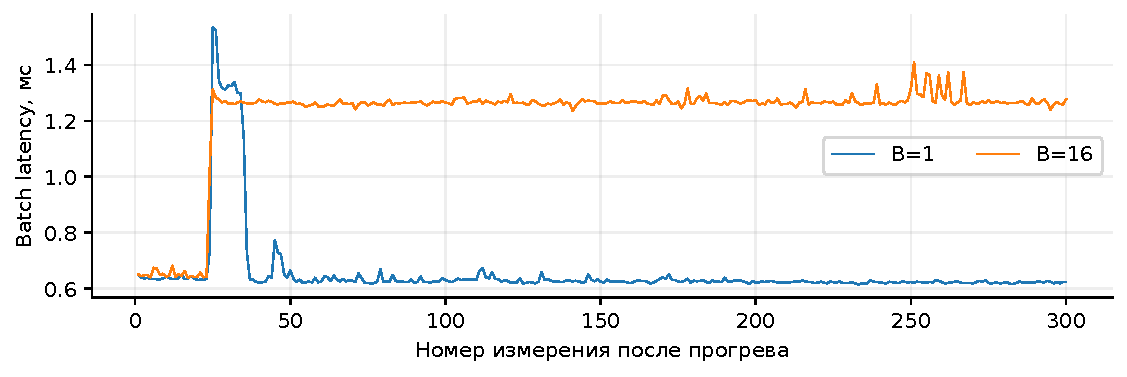
\includegraphics[width=.92\linewidth]{figures/timing_stability.pdf}
\caption{Все 300 измерений дополнительной серии при $B=1$ и $B=16$ (\run{D08}). Выбросы не удалялись.}\label{fig:timing}
\end{figure}

При $B=1$ и $B=16$ CV равен 20.81\% и 13.62\%, то есть порог 10\% не достигнут даже после увеличения числа повторов. Для $B=16$ частота SM изменилась с 1425 до 1620~MHz; для $B=1$ начальная и конечная частоты одинаковы, 1425~MHz. Эти наблюдения согласуются с влиянием режима работы GPU, однако не локализуют все выбросы: отдельно не разделены изменения частоты и задержки запуска со стороны host. Поэтому общая устойчивость latency вне основной серии не установлена. Снижение CV при больших $B$ показывает, что относительная роль накладных расходов уменьшается, но не устраняет указанный отрицательный результат.

\section{Уровни воспроизводимости и обсуждение}
Уровень R0 означает возможность установить происхождение результата, R1 --- восстановить split и входной поток, R2 --- повторить траекторию и итоговую метрику, R3 --- продолжить прерванный опыт эквивалентно непрерывному. Эти уровни относятся к проверенным условиям, а не являются безусловным свойством программы~\cite{lab0}.

В режиме A достигнут R3: \run{R02}/\run{R03} подтверждают повторяемость данных и step loss, а \run{R04}/\run{R06} --- восстановление состояния. В режиме B также наблюдался R3 в пределах заданных допусков, причём фактические расхождения равны нулю (\run{R07}/\run{R08}, \run{R09}/\run{R11}). В режиме C наблюдалось такое же совпадение в конкретной серии (\run{R12}/\run{R13}, \run{R14}/\run{R16}), включая один одинаковый пропуск обновления. Утверждение о C не распространяется на произвольные AMP-, worker- и GPU-условия.

Между A, B и C итоговые accuracy различаются: 0.6232, 0.6182 и 0.6326. Это не противоречит E1, где требуется совпадение повторов внутри одного режима. Переход на устройство или арифметическую точность меняет вычислительную траекторию даже при одинаковом seed. По одному запуску каждого режима нельзя установить превосходство AMP по качеству; эти числа характеризуют проверку воспроизводимости.

E1 и E2 отвечают на разные вопросы. E1 показывает отсутствие вариативности при повторении фиксированного seed; E2 обнаруживает стандартное отклонение 0.008708 при смене seed. Следовательно, детерминизм не устраняет чувствительность обучения к начальным условиям. Равенство конечных accuracy также недостаточно: найденные в вопросе~\ref{cf:4} запуски имеют одинаковую accuracy, но разные значения loss на всех 2016 шагах.

Наконец, воспроизводимость предсказаний и стабильность времени исполнения различны. Для одной и той же модели наблюдалось точное повторение обучения, но дополнительный GPU timing не удовлетворил порогу CV для малых batch. Поэтому вывод R3 не следует интерпретировать как гарантию одинаковой latency или одинаковой вычислительной стоимости на другой машине.

\section{Ответы на контрфактические вопросы}
\subsection{Вопрос 1. Минимальный эффект и число запусков}\label{cf:1}
В основной серии \run{R17}--\run{R21} получены $\overline m=0.633440$ и $s_m=0.008708$. Ориентир задания $2s_m=0.017416$ соответствует 1.742 п.п.; меньший прирост без дополнительной серии нельзя считать установленным. Это эвристика, а не расчёт мощности конкретного статистического теста.

При независимых одинаково распределённых запусках стандартная ошибка среднего равна $s_m/\sqrt N$. Чтобы уменьшить её вдвое при примерно фиксированных квантилях, требуется увеличить число запусков в четыре раза:
\begin{equation}
\frac{s_m}{\sqrt{N_{\text{нов}}}}\approx
\frac12\frac{s_m}{\sqrt N}
\quad\Longrightarrow\quad N_{\text{нов}}\approx4N=20.
\label{eq:power}
\end{equation}
По измерению \run{D01} двадцать запусков по 12 эпох потребовали бы около 96.36~мин; дополнительные 15 --- около 72.27~мин. Это больше исходной оценки 62.63~мин всей обязательной CPU-программы и требует пересмотра бюджета. Число 20 является приближённой оценкой по масштабированию ошибки; для заданной мощности, альтернативы и уровня значимости необходим отдельный план. В рамках этого отчёта новые запуски для проверки мощности не выполнялись.

\subsection{Вопрос 2. Изменение числа workers с 0 на 2}\label{cf:2}
При workers=2 выполнены \run{R22}/\run{R23}; между ними максимальная $\varepsilon_{rel}$ loss и разность accuracy равны нулю. По сравнению с workers=0 (\run{R02}) сохранились split, checksum первого batch и все 2016 step loss; итоговая accuracy во всех трёх случаях равна 0.6232.

В данном pipeline нет случайных аугментаций, порядок объектов задаётся отдельным generator, а workers получают фиксированные seed. Изменение параллелизма загрузки не изменило данные, поступившие в модель. Поэтому в измеренном случае граница повторяемости не была нарушена. Этот результат не гарантирует совпадения при случайных преобразованиях внутри worker или иных правилах выдачи данных.

\subsection{Вопрос 3. Сохранение только весов модели}\label{cf:3}
При продолжении только с \texttt{model.state\_dict()} итоговое расхождение \run{R24} относительно непрерывного \run{R04} составило $\Delta_\theta=0.371028$, тогда как полный resume дал нуль. Итоговая val accuracy усечённого восстановления равна 0.6292; близкая к контрольной метрика не означает совпадения состояния.

Для локализации причин в \run{D03} использованы одна сохранённая точка и один фиксированный градиент: loss контрольного batch равна 1.2374443 и совпадает с первым записанным шагом эпохи 7. Сброс только моментов AdamW при прежней learning rate дал $\Delta_\theta=0.00982349$. Изменение только learning rate с $0.00057115742$ на $0.001$ при сохранённых моментах дало $\Delta_\theta=0.00151970$. Отсутствие состояния generator загрузчика также изменило следующий batch.

Таким образом, память оптимизатора, позиция scheduler и порядок данных являются отдельно проверенными источниками расхождения. Одношаговые эффекты нельзя складывать как разложение конечного $\Delta_\theta$: дальнейшая динамика нелинейна. В этой CNN нет dropout и случайных аугментаций; отдельный вклад глобальных Python/NumPy/Torch RNG в итоговое расхождение здесь не измерялся.

\subsection{Вопрос 4. Одинаковая accuracy при разных траекториях}\label{cf:4}
Среди пяти исходных seed E2 пары с $|\Delta\operatorname{acc}|<0.001$ не оказалось. В сохранённой дополнительной серии по тому же протоколу выполнены три запуска, \run{R25}--\run{R27}. Пара \run{R25}/\run{R27} дала одинаковую val accuracy 0.6364, однако все 2016 значений step loss различаются, максимальная $\varepsilon_{rel}=0.510981$.

Одна итоговая accuracy является сжатым описанием поведения модели: разные параметры, вероятности и решения на отдельных изображениях могут дать одинаковое число правильных ответов. Поэтому она не доказывает воспроизведения траектории. Дополнительные seeds служат контрпримером; они не включены задним числом в среднее, $s_m$ и доверительный интервал основной пятёрки.

\subsection{Вопрос 5. Смена версии cuDNN}\label{cf:5}
В manifest \run{R02} зарегистрирована версия cuDNN 90701. Его EXP\_ID: \nolinkurl{6a750eb4531ac754cde7}. При смене только cuDNN изменится поле окружения \nolinkurl{environment.cudnn}; EXP\_ID при прежних коде, конфигурации, данных и seed останется тем же, поскольку окружение не включается в формулу~\eqref{eq:ids}. Новый запуск всё равно получит новый RUN\_ID.

Регистрация нового окружения сохраняет возможность проследить происхождение результата, то есть R0. Сохранённый split и логика загрузчика позволяют отдельно проверить R1, но R2/R3 после смены библиотеки без новых измерений не гарантируются. Фактическая замена cuDNN в этом опыте не выполнялась; это анализ зарегистрированных полей и границ гарантий, а не утверждение о проверенном обновлении библиотеки.

\subsection{Вопрос 6. Изменение одного байта данных}\label{cf:6}
В \run{D04}/\run{D05} изменён один байт отдельной копии \texttt{data\_batch\_1} при неизменных имени, пути и размере. SHA256 файла изменился с префикса \texttt{54636561a3ce} на \texttt{8b0686ccaea3}. Изменились data fingerprint и EXP\_ID, сохранились config hash, split fingerprint, seed, профиль и состояние исходного кода. RUN\_ID различаются как у любых независимых запусков.

Следовательно, fingerprint по содержимому обнаруживает изменение, которое не обнаружил бы идентификатор, основанный только на пути и размере. Официальные обучающие файлы не изменялись; их проверка MD5 дополнительно отклонила бы повреждённую копию до обучения. Это вмешательство в данные с регистрацией идентичности, а не новая тренировка на повреждённом датасете.

\subsection{Вопрос 7. Первая итерация и прогретая latency}\label{cf:7}
При $B=1$ CPU first forward занял 3.3674~мс, медиана после прогрева --- 1.1524~мс: отношение 2.922 (\run{D06}). На CUDA первая итерация заняла 168.5951~мс против медианы 0.66195~мс, отношение 254.695 (\run{D07}).

Увеличение начального интервала согласуется с ленивой инициализацией вычислительных ресурсов, подготовкой памяти и вычислительных ядер. Без отдельной трассировки нельзя количественно разделить эти составляющие. Поэтому первая итерация не является оценкой установившейся latency; её сохранение отдельно от прогретой серии позволяет увидеть этот эффект, не исключая неудобное наблюдение из результатов.

\subsection{Вопрос 8. Минимум latency и максимум throughput}\label{cf:8}
На CPU минимальная медианная latency равна 1.1524~мс при $B=1$, а максимальный throughput --- 1192.01 объекта/с при $B=64$ (\run{D06}). На CUDA минимум медианной latency также при $B=1$, 0.66195~мс, но максимум throughput достигается при $B=256$ и равен 50\,032.69 объекта/с (\run{D07}). Оптимальные размеры batch не совпали на обоих устройствах.

Latency измеряет ожидание целого batch, throughput --- число обработанных объектов за единицу времени. Увеличение batch распределяет постоянные накладные расходы на большее число изображений и повышает загрузку вычислительных блоков до насыщения. На CPU throughput при $B=256$ уже не выше, чем при $B=64$; статистическая значимость небольшого различия соседних значений отдельно не проверялась. Вывод относится к измеренной сетке batch sizes и данной сети.

\clearpage
\section{Ограничения и заключение}
\subsection{Область применимости результатов}
Повторяемость проверена для одной компактной CNN, одного split и зафиксированного окружения. Перенос на другую версию PyTorch/CUDA/cuDNN, другое устройство или случайные аугментации требует отдельной проверки. Точное восстановление подтверждено на границах полных эпох; произвольное прерывание внутри mini-batch не исследовано. Отсутствие самостоятельного файла split преподавателя не позволяет утверждать побитовое совпадение с ним, хотя численности ролей и процедура зафиксированы.

Основной E2 описывает вариативность пяти заранее заданных seed на одном validation-наборе. Его доверительный интервал не охватывает изменения датасета и не обосновывает универсальную мощность сравнения методов. Дополнительные seeds вопроса~\ref{cf:4} найдены адаптивно и используются только для контрпримера. Результаты test не заявляются, поскольку в Lab~0 они не измерялись.

Основная E4-серия прошла порог CV, однако дополнительная серия при $B=1,16$ его не прошла. Причины нестабильности локализованы лишь частично: наблюдались изменения частоты GPU, но их вклад не отделён от host-задержек. Нельзя заявлять общую стабильность latency вне конкретной серии. Это отрицательное наблюдение сохраняется наряду с положительным результатом повторяемости обучения.

\subsection{Заключение}
Реализован и экспериментально проверен единый жизненный цикл нейросетевого эксперимента: конфигурация, данные, обучение, оценивание, регистрация и восстановление состояния. В окончательном E0 train loss уменьшилась более чем вдвое, val accuracy достигла 62.32\%. Исходная попытка на десяти эпохах порог не выполнила и не заменяется этим положительным результатом.

Повторы внутри A/B/C и полный resume воспроизвели записанные траектории; $\Delta_\theta=0$ во всех трёх режимах в данном окружении. Смена seed дала $63.344\pm0.871\%$ val accuracy при $N=5$, что показывает необходимость повторных запусков для интерпретации небольших улучшений. Усечённый checkpoint привёл к $\Delta_\theta=0.371028$; итоговая accuracy оказалась недостаточным свидетельством воспроизведения. Профилирование подтвердило различие между минимумом latency и максимумом throughput, а дополнительная GPU-серия выявила границы стабильности времени исполнения.

Главный результат работы --- возможность связать каждое численное утверждение с условиями и конкретным запуском и различить воспроизводимость входов, траектории, итоговой метрики и вычислительной стоимости. Достигнутый R3 относится к проверенным режимам и окружению, а не является безусловной гарантией для любых будущих экспериментов.

\Needspace{11\baselineskip}
\renewcommand{\refname}{Список использованных источников}
\begin{thebibliography}{9}
\addcontentsline{toc}{section}{Список использованных источников}
\bibitem{lab0} Лабораторная работа 0. Инфраструктура воспроизводимых экспериментов и единый Experiment Harness. Курс «Нейронные сети». Ред. 2.1 от 09.10.2026. 24 с.\newline
URL: \url{https://drive.google.com/file/d/1LUHswJEcHctLX3C_pi7DFe2Si9lGsxJT/view}\newline
(дата обращения: 03.11.2026).
\bibitem{torch} PyTorch. Reproducibility: документация версии 2.7.\newline
URL: \url{https://docs.pytorch.org/docs/2.7/notes/randomness.html}\newline
(дата обращения: 03.11.2026).
\bibitem{cifar} Krizhevsky A. CIFAR-10 and CIFAR-100 datasets.\newline
URL: \url{https://www.cs.toronto.edu/~kriz/cifar.html}\newline
(дата обращения: 03.11.2026).
\end{thebibliography}

\clearpage
\section*{Приложение А. Идентификация запусков}
\addcontentsline{toc}{section}{Приложение А. Идентификация запусков}
Обозначения R относятся к обучающим запускам, D --- к бюджетному измерению, исходному E0 и дополнительным диагностическим опытам. Прерванные \run{R05}, \run{R10}, \run{R15} завершены на эпохе 6 и являются родителями resume, а не независимыми двенадцатиэпоховыми результатами. Восстановленные \run{R06}, \run{R11}, \run{R16} продолжают соответствующие траектории. Все полные RUN\_ID приведены ниже, чтобы ссылки в результатах и ответах оставались однозначными.
\begingroup\small\setstretch{1.03}\setlength{\tabcolsep}{3pt}\begin{longtable}{@{}l>{\raggedright\arraybackslash}p{3.7cm}p{10.8cm}@{}}
\caption{Обозначения запусков и соответствующие RUN\_ID.}\label{tab:runs}\\
\toprule Код & Условие & RUN\_ID \\ \midrule \endfirsthead
\toprule Код & Условие & RUN\_ID \\ \midrule \endhead
\bottomrule\endfoot
\hypertarget{R01}{R01} & E0 & {\fontsize{9.2}{11}\selectfont\texttt{2e863c4124c6c4321515-f73d8ccc23754fcfa4192ba00946809e}} \\
\hypertarget{R02}{R02} & E1-A-1 & {\fontsize{9.2}{11}\selectfont\texttt{6a750eb4531ac754cde7-b798991a1a7b457cbb0de2144b2a4742}} \\
\hypertarget{R03}{R03} & E1-A-2 & {\fontsize{9.2}{11}\selectfont\texttt{6a750eb4531ac754cde7-6f509e890fd64b608afb1088db8a2887}} \\
\hypertarget{R04}{R04} & E3-A-continuous & {\fontsize{9.2}{11}\selectfont\texttt{6a750eb4531ac754cde7-121bb015882b4809bac8725db13d3585}} \\
\hypertarget{R05}{R05} & E3-A-interrupted & {\fontsize{9.2}{11}\selectfont\texttt{6a750eb4531ac754cde7-780d211ff99d477cabc89ecdd1cd58de}} \\
\hypertarget{R06}{R06} & E3-A-resumed & {\fontsize{9.2}{11}\selectfont\texttt{6a750eb4531ac754cde7-c5ba381370ce489991574e85997b1a8f}} \\
\hypertarget{R07}{R07} & E1-B-1 & {\fontsize{9.2}{11}\selectfont\texttt{24fb5beae9305a2c10aa-de06a13cc7eb402f995f5668a778dfe6}} \\
\hypertarget{R08}{R08} & E1-B-2 & {\fontsize{9.2}{11}\selectfont\texttt{24fb5beae9305a2c10aa-832c4282c2bb4bd6a076707c0f7b83a2}} \\
\hypertarget{R09}{R09} & E3-B-continuous & {\fontsize{9.2}{11}\selectfont\texttt{24fb5beae9305a2c10aa-625428fa57f94801a094c63c66e1ffe6}} \\
\hypertarget{R10}{R10} & E3-B-interrupted & {\fontsize{9.2}{11}\selectfont\texttt{24fb5beae9305a2c10aa-ea45996d25e745f48acfd8b7801c48a0}} \\
\hypertarget{R11}{R11} & E3-B-resumed & {\fontsize{9.2}{11}\selectfont\texttt{24fb5beae9305a2c10aa-c71cd08cb5ce48548549d1375248531b}} \\
\hypertarget{R12}{R12} & E1-C-1 & {\fontsize{9.2}{11}\selectfont\texttt{1e2acbdbd42e2d6577a1-fa3b237cd8c84cea899ea6716c2bf01f}} \\
\hypertarget{R13}{R13} & E1-C-2 & {\fontsize{9.2}{11}\selectfont\texttt{1e2acbdbd42e2d6577a1-5a0fe15af76a434abe485f83138ea1eb}} \\
\hypertarget{R14}{R14} & E3-C-continuous & {\fontsize{9.2}{11}\selectfont\texttt{1e2acbdbd42e2d6577a1-6ca15418d29047f28c044e2c3bc72b60}} \\
\hypertarget{R15}{R15} & E3-C-interrupted & {\fontsize{9.2}{11}\selectfont\texttt{1e2acbdbd42e2d6577a1-0b76c9aae5b743bfb74f968c0a92ace6}} \\
\hypertarget{R16}{R16} & E3-C-resumed & {\fontsize{9.2}{11}\selectfont\texttt{1e2acbdbd42e2d6577a1-bb15ad788cda4f19b0e25eebf5201b6f}} \\
\hypertarget{R17}{R17} & E2-0 & {\fontsize{9.2}{11}\selectfont\texttt{6a750eb4531ac754cde7-1d3687b74ea341a4a1e606a63170cf75}} \\
\hypertarget{R18}{R18} & E2-1 & {\fontsize{9.2}{11}\selectfont\texttt{ffcacb74be86c9753a8d-0dbcbab3f9b2449da8f22b799f36cd6d}} \\
\hypertarget{R19}{R19} & E2-2 & {\fontsize{9.2}{11}\selectfont\texttt{c9425d8eded07ded9b07-9a72d90391944975ad604e0ab77440c9}} \\
\hypertarget{R20}{R20} & E2-3 & {\fontsize{9.2}{11}\selectfont\texttt{39881f615bd21f39c28d-eb622515499c4ca9af7b5541ec08f28d}} \\
\hypertarget{R21}{R21} & E2-4 & {\fontsize{9.2}{11}\selectfont\texttt{cb0f969da6cfc1ee7759-fe0f39acfd234932801e11365501a14a}} \\
\hypertarget{R22}{R22} & CF02-workers-1 & {\fontsize{9.2}{11}\selectfont\texttt{18ba7b9da1c4f164b795-b171839347714fbeac64c77f997c5e85}} \\
\hypertarget{R23}{R23} & CF02-workers-2 & {\fontsize{9.2}{11}\selectfont\texttt{18ba7b9da1c4f164b795-b085a9d3aed8425891c5541ea8a0ac25}} \\
\hypertarget{R24}{R24} & CF03-weights-only & {\fontsize{9.2}{11}\selectfont\texttt{c5efc232293daa65ca54-44bb5d7a874643259168a727c3bb948d}} \\
\hypertarget{R25}{R25} & CF04-extra-1 & {\fontsize{9.2}{11}\selectfont\texttt{640b5fb517c666ee2ce4-2eacc02910704bfbbd95feae4626ba44}} \\
\hypertarget{R26}{R26} & CF04-extra-2 & {\fontsize{9.2}{11}\selectfont\texttt{c25cb47bc0282725a620-214e3871a8e8497487723a62760e2f94}} \\
\hypertarget{R27}{R27} & CF04-extra-3 & {\fontsize{9.2}{11}\selectfont\texttt{e74e6c8aa32ebadb48e5-fdb056f5c03546819b60bcef0a382e86}} \\
\hypertarget{D01}{D01} & Оценка бюджета & {\fontsize{9.2}{11}\selectfont\texttt{e592bd6f1f2da6e9f959-f1f208b3b6844b71a89d774e5e291a44}} \\
\hypertarget{D02}{D02} & Начальный E0, K=10 & {\fontsize{9.2}{11}\selectfont\texttt{187f3bd4a93cd598f53b-47b8eee4daa145949b8406914abff222}} \\
\hypertarget{D03}{D03} & Один шаг: состояние AdamW & {\fontsize{9.2}{11}\selectfont\texttt{699083a5d60b457b7a27-4565dcc8697040c498b47d8fedaae4d4}} \\
\hypertarget{D04}{D04} & Данные до изменения байта & {\fontsize{9.2}{11}\selectfont\texttt{86c8dd0011a17e664ca2-d4864d8b3e2446ebbd586261f081c1b9}} \\
\hypertarget{D05}{D05} & Данные после изменения байта & {\fontsize{9.2}{11}\selectfont\texttt{26fbdb25ae58f6ba17cc-acc3b6459ddd475885825852351b1aa8}} \\
\hypertarget{D06}{D06} & E4, CPU, N=100 & {\fontsize{9.2}{11}\selectfont\texttt{c29fec693e78f31bd03b-2afa25ee666d4ce4823bf95d43f5c1a8}} \\
\hypertarget{D07}{D07} & E4, CUDA, N=100 & {\fontsize{9.2}{11}\selectfont\texttt{724bae602e86195355ad-dbf545e3a7da421e9daf3626733fb95d}} \\
\hypertarget{D08}{D08} & E4, CUDA, N=300 & {\fontsize{9.2}{11}\selectfont\texttt{efe887782e2794dfe859-e0ce03d1443a4128b6f5749b42fcc1fb}} \\
\end{longtable}\endgroup
